
\chapter{Evaluation of Accuracy in Heart Rate Determination using Samsung Gear S3 Smartwatch BVP data}

\section{Objective}

This experiment aims to conclude on the reliability of Samsung Gear Gear Smartwatch Photoplethysmography sensor (PPG) as a way to determine heart rate (HR).
In order to determine the accuracy of HR given by Gear, a BitAlino based chest-band was used, to acquire ECG simultaneously to the collection of PPG, and provide a ground-truth for heart rate. Besides Gear's HR calculation, an onset detection algorithm was also used to determine HR from PPG data.

\section{Experimental Procedure}

Three young subjects volunteered to this evaluation and data was collected in different situations from both ECG and PPG sensors:
\begin{description}[labelindent=\parindent]
	\item[--] 2 minutes resting, with the arm where the Gear was placed being completely still;
	\item[--] 5 minutes walking at a regular pace;
	\item[--] \(\sim\)2 hours where the subjects were told to behave like they normally would in their day-to-day life
\end{description}

\noindent

To guarantee consistency in results, the resting and walking experiments were repeated with two of the subjects for 5 and 10 minutes, respectively.

Heart rate was calculated in 10s windows using three different methods:
	
\begin{description}[labelindent=\parindent]
	\item[--] ECG signal was filtered and segmented in order to locate the R-peak and calculate HR. Filtering stage was composed of a median filter, a low-pass filter and a second median filter;
	\item[--] PPG signal was filtered, segmented and finally an onset detector was used to identify beats;
	\item[--] PPG was used by the Gear pre-implemented algorithm to internally produce a value of HR (the methods used to this are not known);
\end{description}

These methods were applied in each 10s window to allow an estimation of instantaneous HR, that is updated every 10s.

During all the experiments, 3axis accelerometry from the Gear was collected. This had the objective of determining if the increase in movement, induced a larger error in HR determination, by the introduction of motion artifacts (MA) in the PPG signal. From the raw accelerometry signal, the Total energy was calculated according with \Cref{eq:acc_energy}, to provide an heuristic on the "quantity of movement" at wrist level.

\begin{equation}
	E_{ACC}(n)= {{ACC}_{x}(n)}^{2}+{{ACC}_{y}(n)}^{2}+{{ACC}_{z}(n)}^{2}
	\label{eq:acc_energy}
\end{equation}


\FloatBarrier

\section{Results}

\subsection{Rest and walking}



\begin{figure}[!h]
	\centering
	\makebox[\linewidth][c]{%
		\begin{subfigure}[t]{0.55\textwidth}
			\centering
			\captionsetup{width=.75\linewidth}
			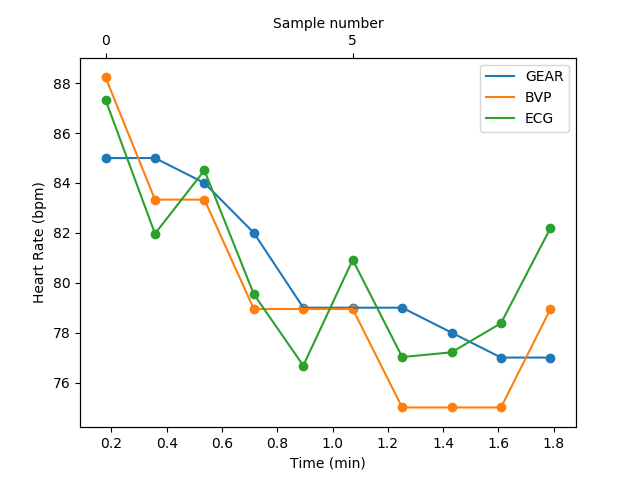
\includegraphics[width=\textwidth]{hr-andre-repouso.png}
			\caption{Heart Rate (Subject 1 resting)}
		\end{subfigure}%
		\begin{subfigure}[t]{0.55\textwidth}
			\centering
			\captionsetup{width=.75\linewidth}
			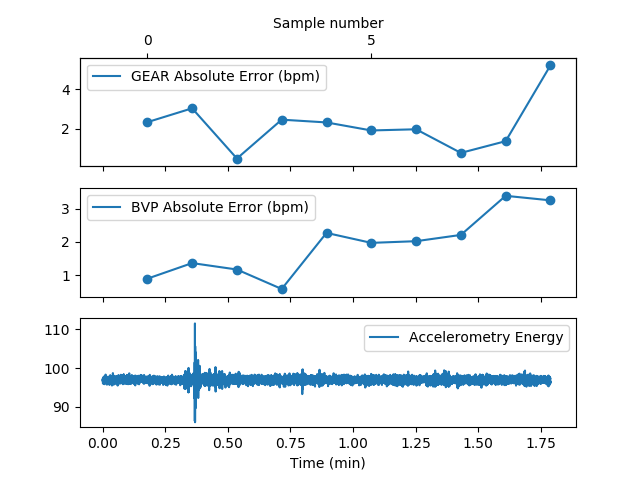
\includegraphics[width=\textwidth]{erro-andre-repouso.png}
			\caption{Absolute error and total accelerometry power (Subject 1 resting)}
		\end{subfigure}%
	}\\
	\makebox[\linewidth][c]{%
		\begin{subfigure}[t]{0.55\textwidth}
			\centering
			\captionsetup{width=.75\linewidth}
			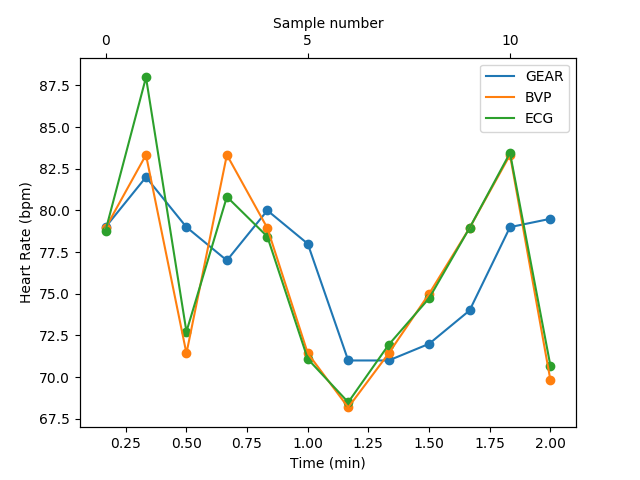
\includegraphics[width=\textwidth]{hr-rita-repouso.png}
			\caption{Heart Rate (Subject 2 resting)}
		\end{subfigure}%
		\begin{subfigure}[t]{0.55\textwidth}
			\centering
			\captionsetup{width=.75\linewidth}
			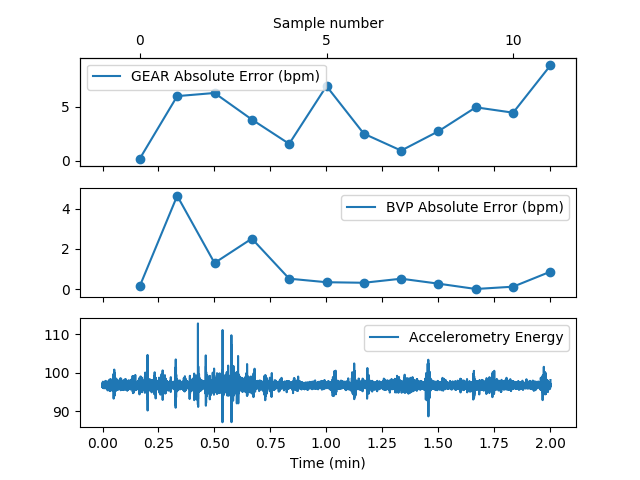
\includegraphics[width=\textwidth]{erro-rita-repouso.png}
			\caption{Absolute error and total accelerometry power (Subject 2 resting)}
		\end{subfigure}%
	}\\
	\makebox[\linewidth][c]{%
		\begin{subfigure}[t]{0.55\textwidth}
			\centering
			\captionsetup{width=.75\linewidth}
			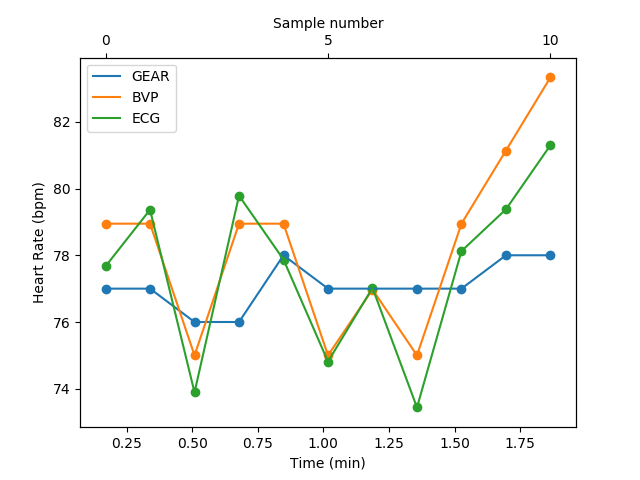
\includegraphics[width=\textwidth]{hr-miguel-repouso.png}
			\caption{Heart Rate (Subject 3 resting)}
		\end{subfigure}%
		\begin{subfigure}[t]{0.55\textwidth}
			\centering
			\captionsetup{width=.75\linewidth}
			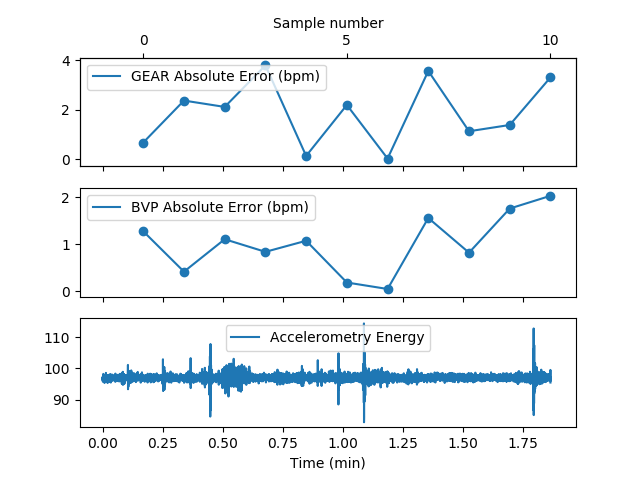
\includegraphics[width=\textwidth]{erro-miguel-repouso.png}
			\caption{Absolute error and total accelerometry power (Subject 3 resting)}
		\end{subfigure}	%
	}\\
	\caption{HR determined using different methods and the erors associated}
	\label{fig:rest}
\end{figure}

\begin{figure}[!h]
	\centering
	\makebox[\linewidth][c]{%
		\begin{subfigure}[t]{0.55\textwidth}
			\centering
			\captionsetup{width=.75\linewidth}
			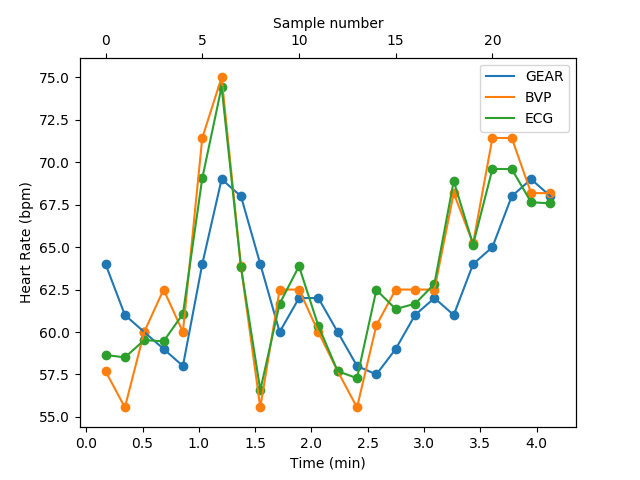
\includegraphics[width=\textwidth]{hr-andre-repouso-longo.png}
			\caption{Heart Rate (Repetition: Subject 1 resting)}
		\end{subfigure}%
		\begin{subfigure}[t]{0.55\textwidth}
			\centering
			\captionsetup{width=.75\linewidth}
			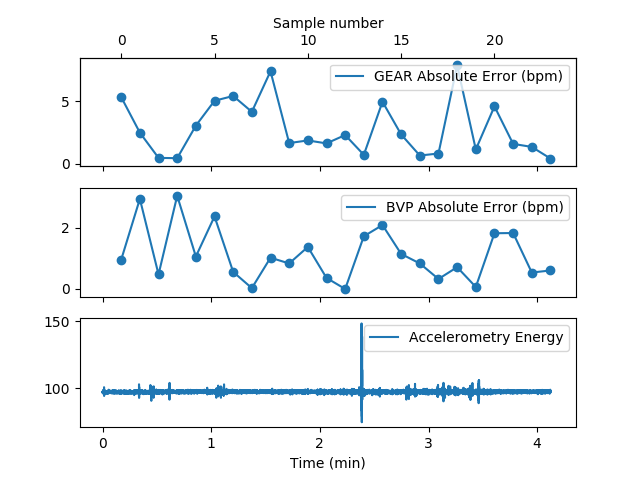
\includegraphics[width=\textwidth]{erro-andre-repouso-longo.png}
			\caption{Absolute error and total accelerometry error (Repetition: Subject 1 resting)}
		\end{subfigure}%
	}\\
	\makebox[\linewidth][c]{%
		\begin{subfigure}[t]{0.55\textwidth}
			\centering
			\captionsetup{width=.75\linewidth}
			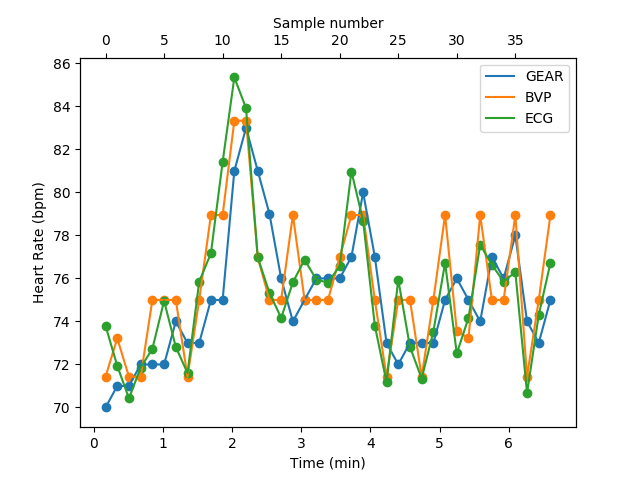
\includegraphics[width=\textwidth]{hr-miguel-repouso-longo.png}
			\caption{Heart Rate (Repetition: Subject 1 resting)}
		\end{subfigure}%
		\begin{subfigure}[t]{0.55\textwidth}
			\centering
			\captionsetup{width=.75\linewidth}
			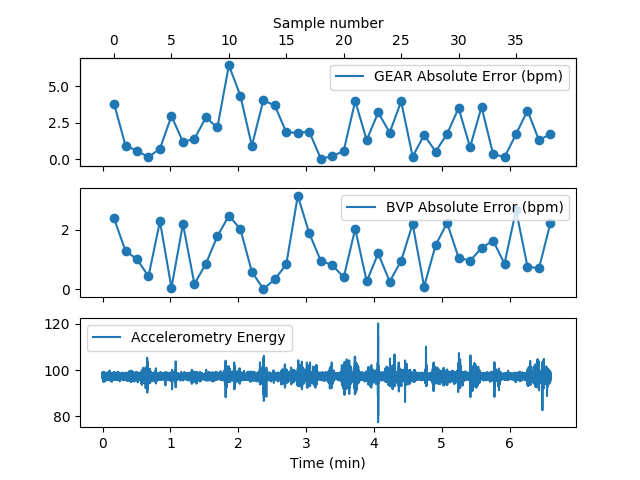
\includegraphics[width=\textwidth]{erro-miguel-repouso-longo.png}
			\caption{Absolute error and total accelerometry error (Repetition: Subject 3 resting)}
		\end{subfigure}%
	}\\	
	\caption{HR determined using different methods and the erors associated}
	\label{fig:rest2}
\end{figure}

\begin{figure}[!h]
	\centering
	\makebox[\linewidth][c]{%
		\begin{subfigure}[t]{0.55\textwidth}
			\centering
			\captionsetup{width=.75\linewidth}
			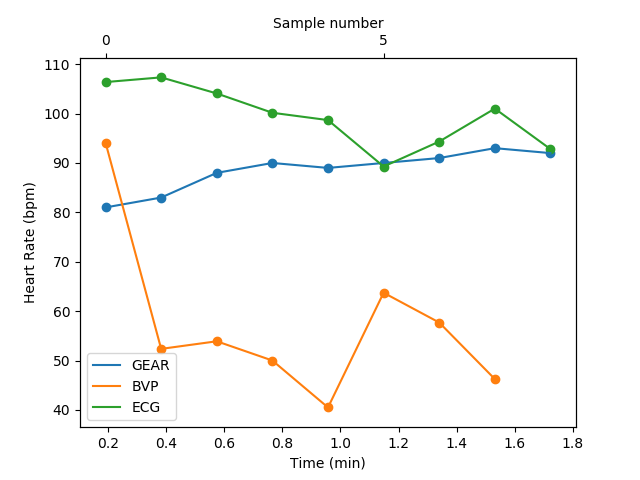
\includegraphics[width=\textwidth]{hr-andre-marcha.png}
			\caption{Heart Rate (Subject 1 walking)}
			\label{fig:walking-1}
		\end{subfigure}%
		\begin{subfigure}[t]{0.55\textwidth}
			\centering
			\captionsetup{width=.75\linewidth}
			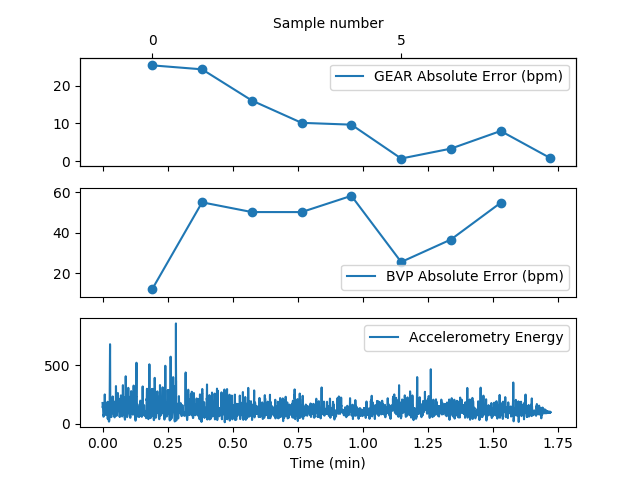
\includegraphics[width=\textwidth]{erro-andre-marcha.png}
			\caption{Absolute error and total accelerometry error (Subject 1 walking)}
		\end{subfigure}%
	}\\
	\makebox[\linewidth][c]{%
		\begin{subfigure}[t]{0.55\textwidth}
			\centering
			\captionsetup{width=.75\linewidth}
			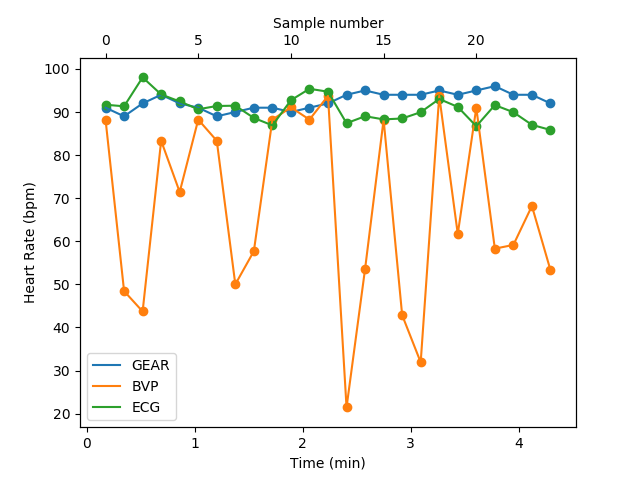
\includegraphics[width=\textwidth]{hr-rita-marcha.png}
			\caption{Heart Rate (Subject 2 walking)}
		\end{subfigure}%
		\begin{subfigure}[t]{0.55\textwidth}
			\centering
			\captionsetup{width=.75\linewidth}
			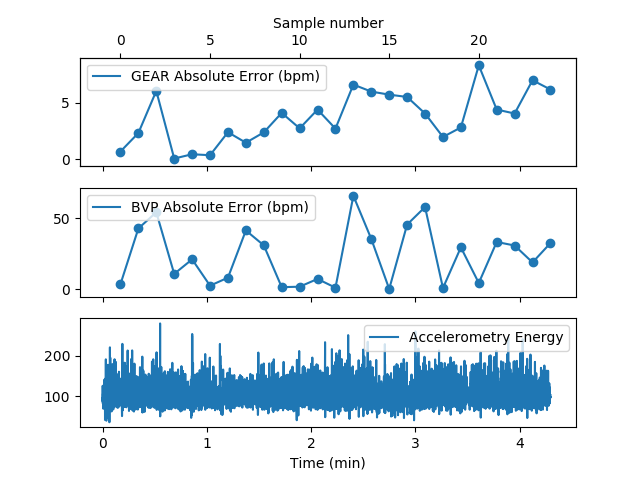
\includegraphics[width=\textwidth]{erro-rita-marcha.png}
			\caption{Absolute error and total accelerometry error (Subject 2 walking)}
		\end{subfigure}%
	}\\
	\makebox[\linewidth][c]{%
		\begin{subfigure}[t]{0.55\textwidth}
			\centering
			\captionsetup{width=.75\linewidth}
			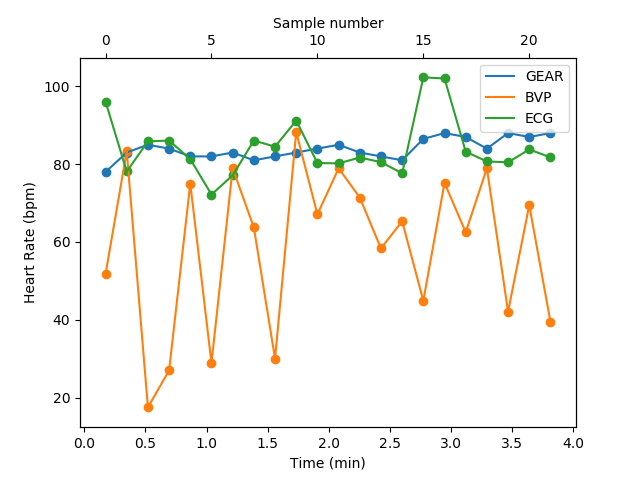
\includegraphics[width=\textwidth]{hr-miguel-marcha.png}
			\caption{Heart Rate (Subject 3 walking)}
			\label{fig:walking-3}
		\end{subfigure}%
		\begin{subfigure}[t]{0.55\textwidth}
			\centering
			\captionsetup{width=.75\linewidth}
			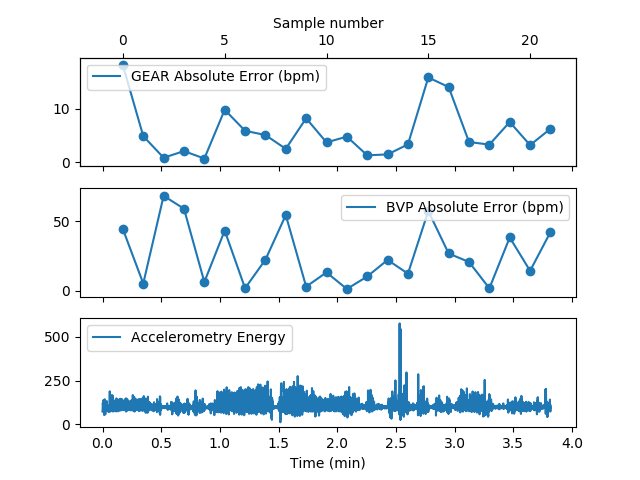
\includegraphics[width=\textwidth]{erro-miguel-marcha.png}
			\caption{Absolute error and total accelerometry error (Subject 3 walking)}
		\end{subfigure}%
	}\\	
	\caption{Absolute Error calculated assuming HR from ECG as ground-truth.}
	\label{fig:walking}
\end{figure}

\begin{figure}[!h]
	\centering
	\makebox[\linewidth][c]{%
		\begin{subfigure}[t]{0.55\textwidth}
			\centering
			\captionsetup{width=.75\linewidth}
			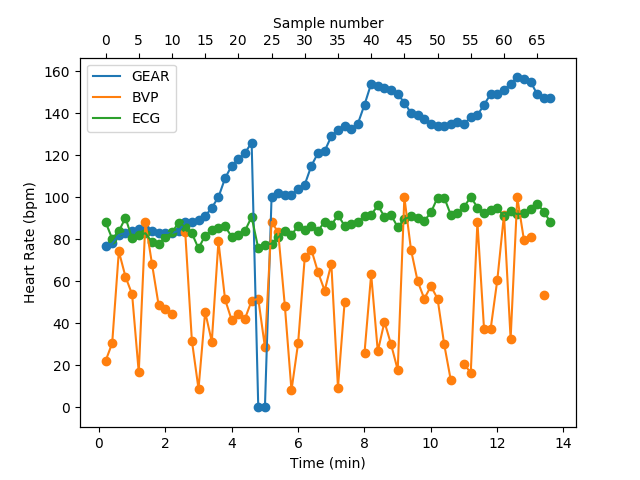
\includegraphics[width=\textwidth]{hr-andre-marcha-longo.png}
			\caption{Heart Rate (Repetition: Subject 1 walking)}
		\end{subfigure}%
		\begin{subfigure}[t]{0.55\textwidth}
			\centering
			\captionsetup{width=.75\linewidth}
			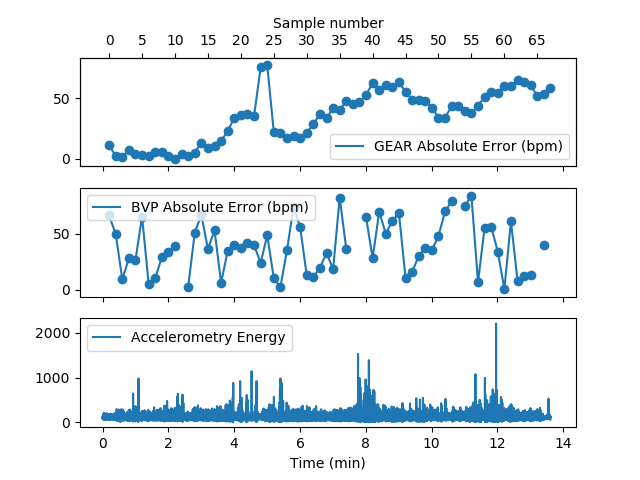
\includegraphics[width=\textwidth]{erro-andre-marcha-longo.png}
			\caption{Absolute error and total accelerometry error (Repetition: Subject 1 walking)}
			\label{fig:walking2-2}
		\end{subfigure}%
	}\\
	\makebox[\linewidth][c]{%
		\begin{subfigure}[t]{0.55\textwidth}
			\centering
			\captionsetup{width=.75\linewidth}
			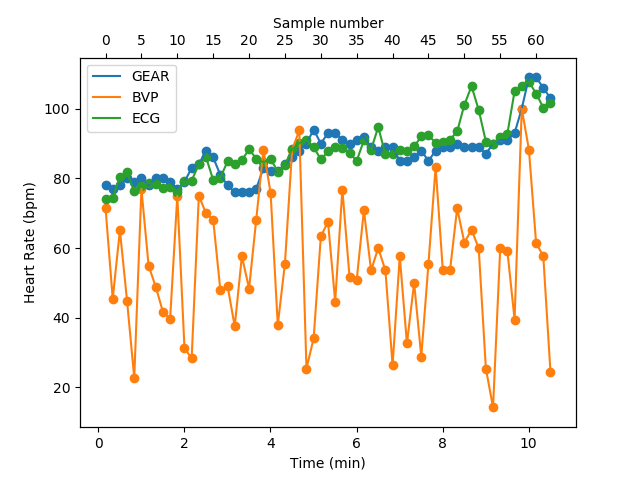
\includegraphics[width=\textwidth]{hr-miguel-marcha-longo.png}
			\caption{Heart Rate (Repetition: Subject 3 walking)}
		\end{subfigure}%
		\begin{subfigure}[t]{0.55\textwidth}
			\centering
			\captionsetup{width=.75\linewidth}
			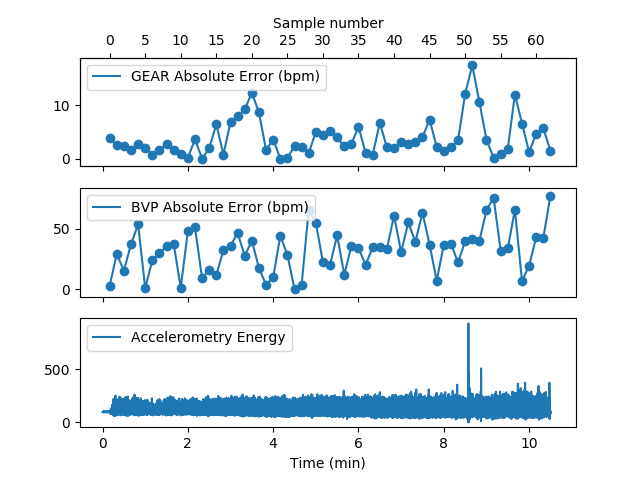
\includegraphics[width=\textwidth]{erro-miguel-marcha-longo.png}
			\caption{Absolute error and total accelerometry error (Repetition: Subject 3 walking)}
		\end{subfigure}%
	}\\	
	\caption{Absolute Error calculated assuming HR from ECG as ground-truth.}
	\label{fig:walking2}
\end{figure}

\begin{equation}
	RMSE_{device}= \sqrt{\frac{1}{N}\sum\limits_{i=1}^N{(HR_{i_{device}}-HR_{i_{ECG}})}}
	\label{eq:rmse}
\end{equation}

\begin{table}[h]
	\centering
	\caption{Root Mean Squared Error \cref{eq:rmse} from each of the subjects (S1, S2, S3) and the average RMS (AV) over the three subjects, when HR is calculated either from the raw BVP signal or by the Gear}
	\label{table:error}
	\begin{tabular}{cc|c|c|c|c|c|c|}
		\cline{3-8}
		&      & S1    & S2    & S3  & S1 (2nd)  & S3 (2nd) & \textbf{AV}    \\ \hline
		\multicolumn{1}{|c|}{\multirow{2}{*}{Rest}} & BVP  & 2.1   & 1.6  & 1.2   & 1.4  & 1.5   & \textbf{1.6}  \\ \cline{2-8} 
		\multicolumn{1}{|c|}{}                      & Gear & 2.5  & 4.8  & 2.3   & 3.6  & 2.5  & \textbf{3.1}  \\ \hline
		\multicolumn{1}{|c|}{\multirow{2}{*}{Walking}} & BVP  & 42.9 & 30.7 & 33.3  & 42.3  & 37.9  & \textbf{46} \\ \cline{2-8} 
		\multicolumn{1}{|c|}{}                      & Gear & 14.0 & 4.3  & 7.4  & 41.12  &  5.2  & \textbf{36}  \\ \hline
	\end{tabular}
\end{table}

Analyzing the plots in \Cref{fig:rest,fig:rest2,fig:walking,fig:walking2}, it is easy to notice that the error in determining the HR while walking is far larger than during rest, which is made clear by the RMS error values in \Cref{table:error}. 

Another conclusion is that the calculation made with the onset detector, although working slightly better in rest, is much worse when the subject is walking. And despite Gear's calculation being more precise than the latter at rest state, there is still a non-negligible error in Gear's automatic calculation. This error becomes significantly worse when there are periods of maintained activity, as can be seen in \Cref{fig:walking2-2}, where the subject's accelerometry energy is elevated during the entire experiment, and the MA induced in BVP signal, lead to a very large error in HR determination.


\FloatBarrier
\pagebreak

\subsection{Event Detection}

\begin{figure}[!h]
	\centering
	\makebox[\linewidth][c]{%
		\begin{subfigure}[t]{0.55\textwidth}
			\centering
			\captionsetup{width=.75\linewidth}
			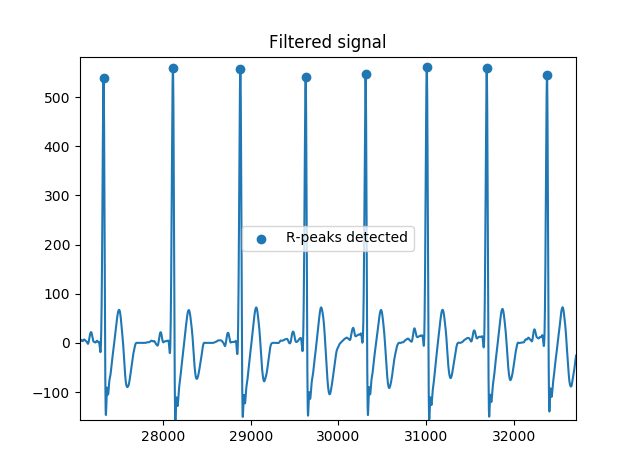
\includegraphics[width=\textwidth]{repouso-ecg.png}
			\caption{Segment of ECG signal with the detected R-peaks during rest}
		\end{subfigure}%
		\begin{subfigure}[t]{0.55\textwidth}
			\centering
			\captionsetup{width=.75\linewidth}
			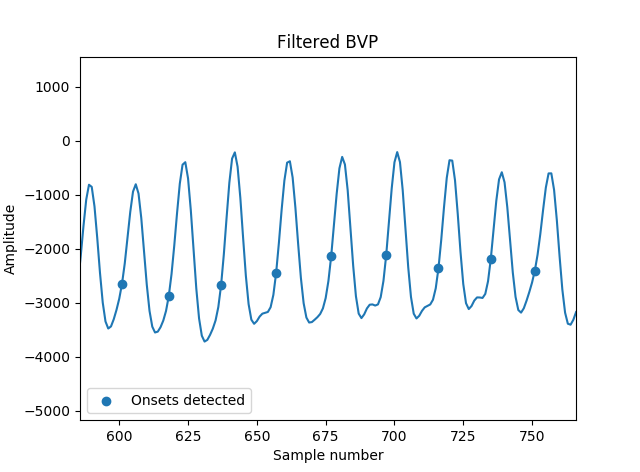
\includegraphics[width=\textwidth]{repouso-bvp.png}
			\caption{Segment of BVP signal with the detected onsets during rest}
		\end{subfigure}%
	}\\
	\makebox[\linewidth][c]{%
		\begin{subfigure}[t]{0.55\textwidth}
			\centering
			\captionsetup{width=.75\linewidth}
			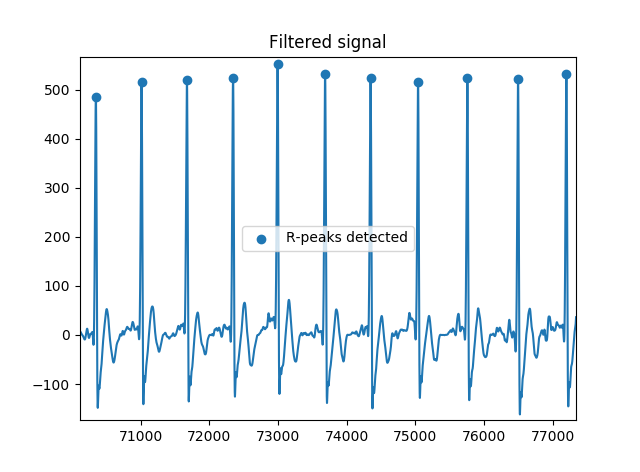
\includegraphics[width=\textwidth]{marcha-ecg.png}
			\caption{Segment of ECG signal with the detected R-peaks while walking}
		\end{subfigure}%
		\begin{subfigure}[t]{0.55\textwidth}
			\centering
			\captionsetup{width=.75\linewidth}
			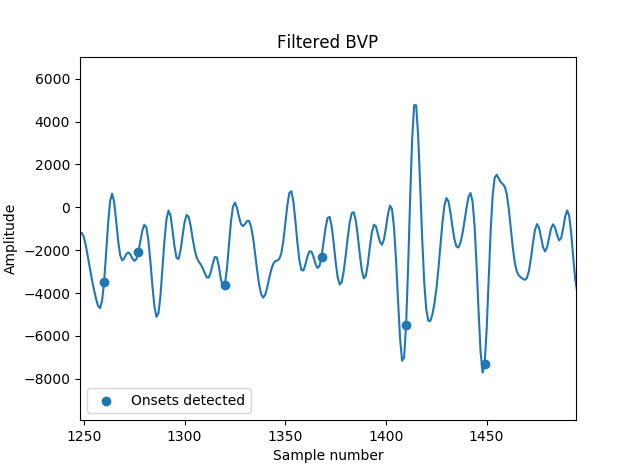
\includegraphics[width=\textwidth]{marcha-bvp.png}
			\caption{Segment of BVP signal with the detected onsets while walking}
		\end{subfigure}%
	}\\
	\caption{Raw ECG and BVP signals and the respective events detected when resting and walking}
	\label{fig:events}
\end{figure}


\begin{table}[!h]
	\centering
	\caption{Number of detected beats in each activity and ratio between $ \# $beats in ECG and BVP}
	\label{table:beats}
	\begin{tabular}{cc|c|c|c|c|}
		\cline{3-6}
		&                & S1            & S2            & S3            & AV            \\ \hline
		\multicolumn{1}{|c|}{\multirow{3}{*}{Rest}}    & BVP            & 137           & 145           & 142           & 141           \\ \cline{2-6} 
		\multicolumn{1}{|c|}{}                         & ECG           & 137           & 154           & 145           & 145           \\ \cline{2-6} 
		\multicolumn{1}{|c|}{}                         & \textbf{Ratio} & \textbf{1}    & \textbf{0.94} & \textbf{0.97} & \textbf{0.91} \\ \hline
		\multicolumn{1}{|c|}{\multirow{3}{*}{Walking}} & ECG            & 127           & 191           & 152           & 157           \\ \cline{2-6} 
		\multicolumn{1}{|c|}{}                         & Gear           & 402           & 387           & 348           & 379           \\ \cline{2-6} 
		\multicolumn{1}{|c|}{}                         & \textbf{Ratio} & \textbf{0.32} & \textbf{0.5}  & \textbf{0.44} & \textbf{0.42} \\ \hline
	\end{tabular}
\end{table}


As it can be observed in \Cref{fig:events} the detection of events while in rest works very well for both the chest-band ECG and the wrist BVP. 

On the other hand, when subject moves, this detection is much harder due to MA corrupting the BVP signal and thus, making the task of detecting the beat onset very hard. This does not occur with the ECG signal since the chest-band is far less sensible to artifacts, having a higher SNR.

These conclusions are corroborated by \Cref{table:beats} where a clear difference in detection performance is obvious. Near 100\% of beats are detected in the BVP signal when resting, whereas, the percentage drops to less than a half when walking. This confirms the poor performance of the onset detection algorithm in the presence of MA.

In \Cref{fig:zoom}, examples of raw signal windows used to calculate HR can be seen, each illustrating a different situation. 

In \Cref{fig:zoom1} is the signal used to calculate sample 15 of the experiment where S3 was walking. As \Cref{fig:walking-3} shows, in this instance HR has a rapid increase, while Gear's estimation remains almost constant, demonstrating Gear's poor ability to deal with rapid changes in HR. 

In \Cref{fig:zoom2}, a very different situation is depicted. Here Gear's error is fairly small and BVP error is very big. This figure contains the raw signal used to calculate the sample nr 2 in \Cref{fig:walking-3}. Here the "quantity of movement" detected was relatively low and HR was fairly constant. This demonstrates that, when the subject is not moving very much, Gear's calculation is relatively accurate, which is not true for onset detection algorithm that has a large error with the slightest movement.

Finally \Cref{fig:zoom3} corresponds to a situation with large error in both methods. This is due, again, to the introduction of MA in the BVP signal.

An observation that can be made from all this examples, is that a peak in accelerometry energy, induces invariably a disruption in the BVP signal, that is amplified by the filtration used. This supports the hypothesis of high correlation level existing between movement, and deterioration of SNR in BVP.



\begin{figure}[!h]
	\centering
	\begin{subfigure}[t]{0.5\textwidth}
		\centering
		\captionsetup{width=.8\linewidth}
		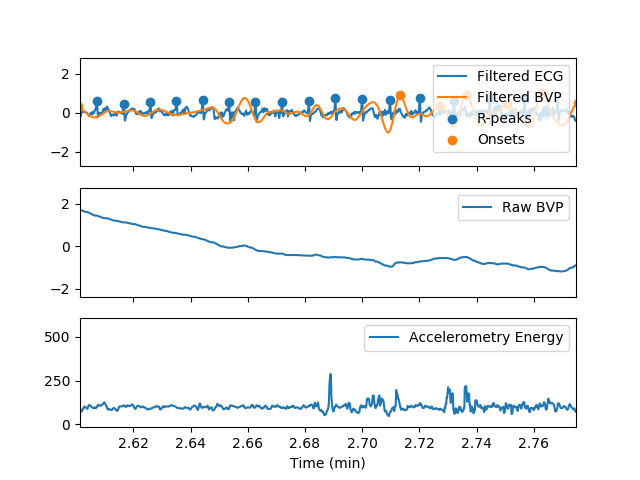
\includegraphics[width=\textwidth]{zoom-miguel-marcha-15.png}
		\caption{Raw signal used to determine sample nr 15 of Subject 3 heart rate while walking. BVP error: 57.5bpm; Gear error: 15.8bpm}
		\label{fig:zoom1}
	\end{subfigure}%
	\begin{subfigure}[t]{0.5\textwidth}
		\centering
		\captionsetup{width=.8\linewidth}
		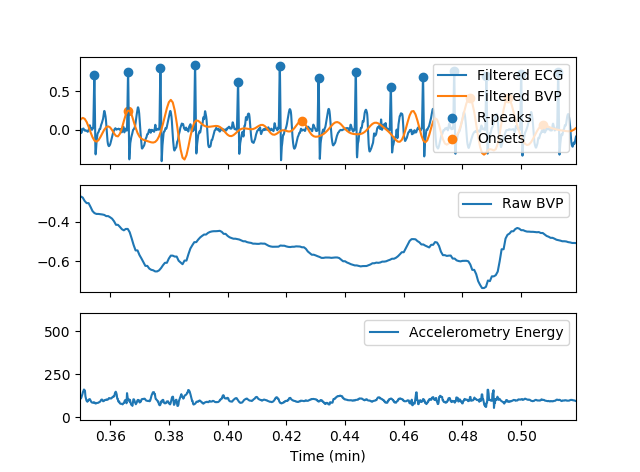
\includegraphics[width=\textwidth]{zoom-miguel-marcha-2.png}
		\caption{Raw signal used to determine sample nr 2 of Subject 3 heart rate while walking. BVP error: 60.4bpm; Gear error: 0.85bpm}
		\label{fig:zoom2}
	\end{subfigure}%
	\vskip 8pt
	\begin{subfigure}[t]{0.5\textwidth}
		\centering
		\captionsetup{width=.8\linewidth}
		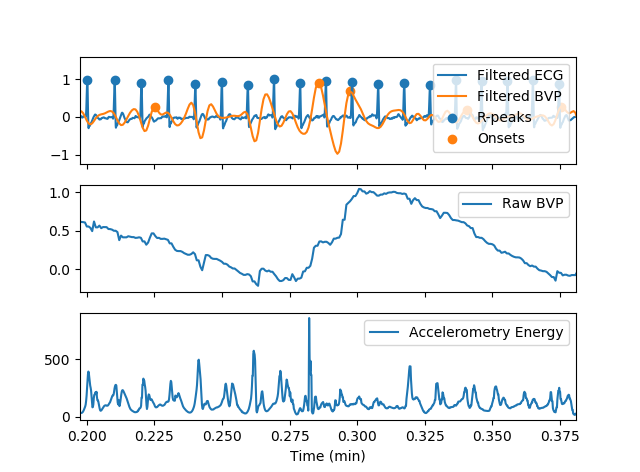
\includegraphics[width=\textwidth]{zoom-andre-marcha-1.png}
		\caption{Raw signal used to determine sample nr 1 of Subject 1 heart rate while walking. BVP error: 54.9bpm; Gear error: 24.3bpm}
		\label{fig:zoom3}
	\end{subfigure}%
	
	\caption{Examples of raw signal windows used to calculate heart rate samples and the simultaneously acquired accelerometry}
	\label{fig:zoom}
\end{figure}


\FloatBarrier
\pagebreak

\subsection{"Real life" case}


\begin{figure}[!h]
	\centering
	\makebox[\linewidth][c]{%
	\begin{subfigure}[t]{0.55\textwidth}
		\centering
		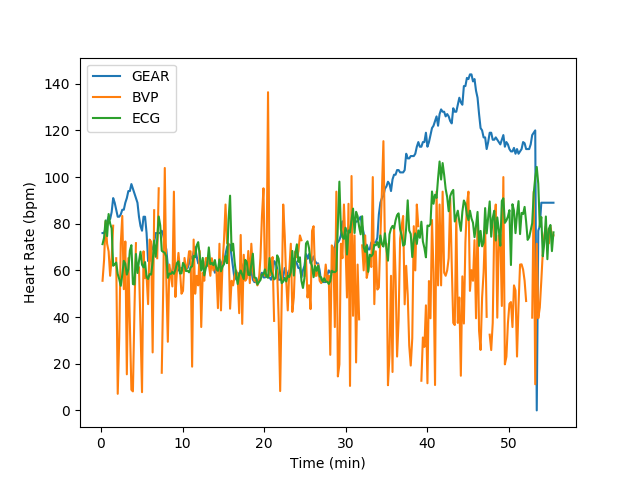
\includegraphics[width=\textwidth]{hr-andre-continuo.png}
		\caption{Subject 1 HR}
	\end{subfigure}%
	\begin{subfigure}[t]{0.55\textwidth}
		\centering
		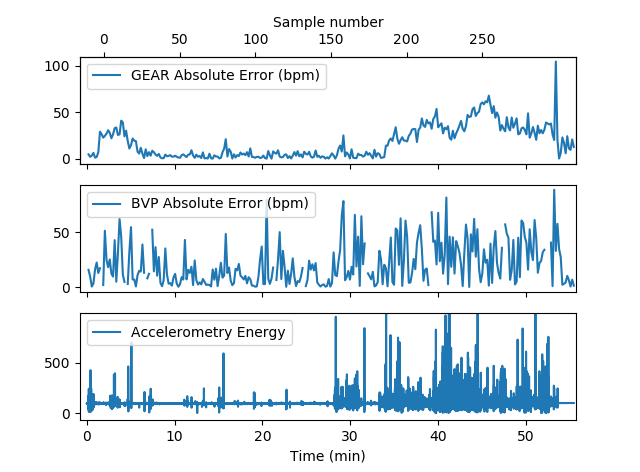
\includegraphics[width=\textwidth]{erro-andre-continuo.png}
		\caption{Subject 1 Absolute Error and Accelerometry Energy}
		\label{fig:real-acc1}
	\end{subfigure}%
	}\\
	\makebox[\linewidth][c]{%
	\begin{subfigure}{0.55\textwidth}
		\centering
		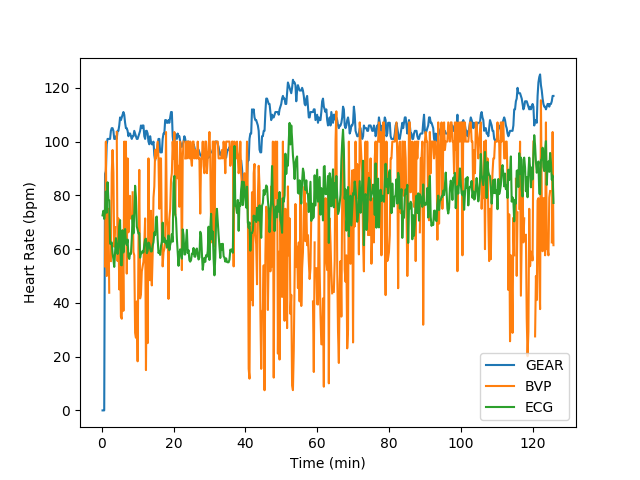
\includegraphics[width=\textwidth]{hr-rita-continuo.png}
		\caption{Subject 2 HR}
	\end{subfigure}%	
	\begin{subfigure}{0.55\textwidth}
		\centering
		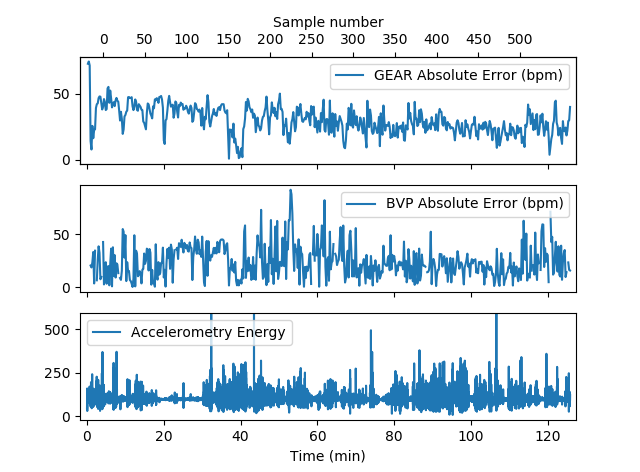
\includegraphics[width=\textwidth]{erro-rita-continuo.png}
		\caption{Subject 2 Absolute Error and Accelerometry Energy}
		\label{fig:real-acc2}
	\end{subfigure}%
	}\\
	\caption{HR and squared error during a segment of the subjects' daily life}
	\label{fig:real}
\end{figure}

\begin{table}[!h]
	\label{table:real}
	\centering
	\caption{Root Mean Squared error from each of the subjects (S1, S2, S3) and the average RMS (AV) when HR is calculatd from the raw BVP signal and by the Gear}
	\begin{tabular}{l|l|l|l|l|}
		\cline{2-5}
		& S1    & S2 & S3    & \textbf{AV}    \\ \hline
		\multicolumn{1}{|l|}{BVP}  & 17.39 & -- & 24.51 & \textbf{20.95} \\ \hline
		\multicolumn{1}{|l|}{Gear} & 31.23 & -- & 26.99 & \textbf{29.11} \\ \hline
	\end{tabular}
\end{table}

\FloatBarrier


It is possible to observe that the determination of HR during the subjects' daily-life presents a considerable amount of error. The HR instantaneous error reached a very high value of more than 40bpm. On top of this high instantaneous error, the average error is also relatively high, reaching 16bpm, indicating the calculation is untrustworthy during most of the acquisition time.

On top of this, it is possible to observe in \Cref{fig:real-acc1} and \ref{fig:real-acc2}, that an increase in movement, (indicated by the larger accelerometry energy) is associated with an increase in Gear's error. This is visible in \Cref{fig:real-acc1} where a region of significant and maintained increase in error, coincides with a period of higher accelerometry energy.

Also in \Cref{fig:real-acc2} the subject kept a high level of activity and the error was considerable. Demonstrating a clear relation between "quantity of movement" and error. Being the only explanation for this, the high corruption of the BVP signal, by the introduction of MA.

\section{Conclusions}



The results of this analysis, clearly indicate that the Gear's automatic calculations and the BVP onset detection are not enough to guarantee accuracy in HR determination for long term studies, especially if the subject is moving. The main reason for this methods' failure is the poor capacity to deal with motion artifacts, conclusion that is supported by the relatively small error when the subject is resting, that increases dramatically when in movement.


A possible strategy to deal with this problem, may be, using an algorithm that takes accelerometry into account and tries to remove movement artifacts and get a denoised BVP signal, with better SNR.
